\chapter[Integrated Detector Commissioning]{Integrated Detector Commissioning}
\label{IDC}

% editing Tex in Atom
% http://rolflekang.com/writing-latex-in-atom/

%Feynman: "all things are made of atoms..."

% If, in some cataclysm, all of scientific knowledge were to be destroyed, and only one sentence passed on to the next generation of creatures, what statement would contain the most information in the fewest words? I believe it is the atomic hypothesis that all things are made of atoms — little particles that move around in perpetual motion, attracting each other when they are a little distance apart, but repelling upon being squeezed into one another. In that one sentence, you will see, there is an enormous amount of information about the world, if just a little imagination and thinking are applied.

% TODO
% SCattering
% * diagram of IFO with scattering illustrated
% * put equations in the sections
% * plot of all of the sources
%
% People
% * Training
% * Visiting - exchange of information
% * Projects for PhD students and postdocs and undergrads
% * balance between project work and scientific research
% * collaboration with other fields: controls, materials, astro, GR, lasers
%
% Figures
% -- interactions: less wacky, B&W
% -- noise budgets: B&W, less busy
% -- Risk: keep?
% -- seismo: B&W
% -- PEM: B&W
%


\section{Introduction}
\label{sec7.1}
If civilization were to be wiped out and only a single statement could be left
carved in stone for future scientists to use, as they rebuilt civilization and
invented gravitational wave detectors to reach out into the universe,
it would be this:

"Think carefully and holistically about your detector before building it
such that no part is neglected as being too small or  coupling at 'second order',
yea, for even the mighty may be brought low by the loose beam dump or the
unforseen cross-coupling."

The interferometer commissioning process has taught us that we could improve
our design process.

We might divide things into subsystems as done in the chapters of a book,
but then to make them work together things are not so orthogonal.
Controllability is much more important than the last few percent of
isolation or noise performance.

It is not wise to design for a single point in parameter space: if each
part of the interferometer can only work when all other pieces are
performing as designed, it becomes impossible to integrate. This phase
space nirvana cannot be reached.

Its the inverse of a Sherlock Holmes locked-room mystery story.

In this chapter we will explore some of the interesting interaction between
disparate sub-systems which make the interferometer commissioning experience
so rich, challenging, and rewarding.


\section{Sub-system Integration Issues}
We design the individual components of the interfererometer to fulfill some
primary goals with some secondary considerations.

But in some cases, the most important driver in the design should, in fact, be the
interaction that this 'isolated' component has with the full system. In some cases,
this interaction is only apparent with the highest circulating laser power levels
and only when considering the smallest mirror displacements.

In the following sections we explore a few examples of this kind of surprising
interaction.


\begin{figure}[h]
\centering
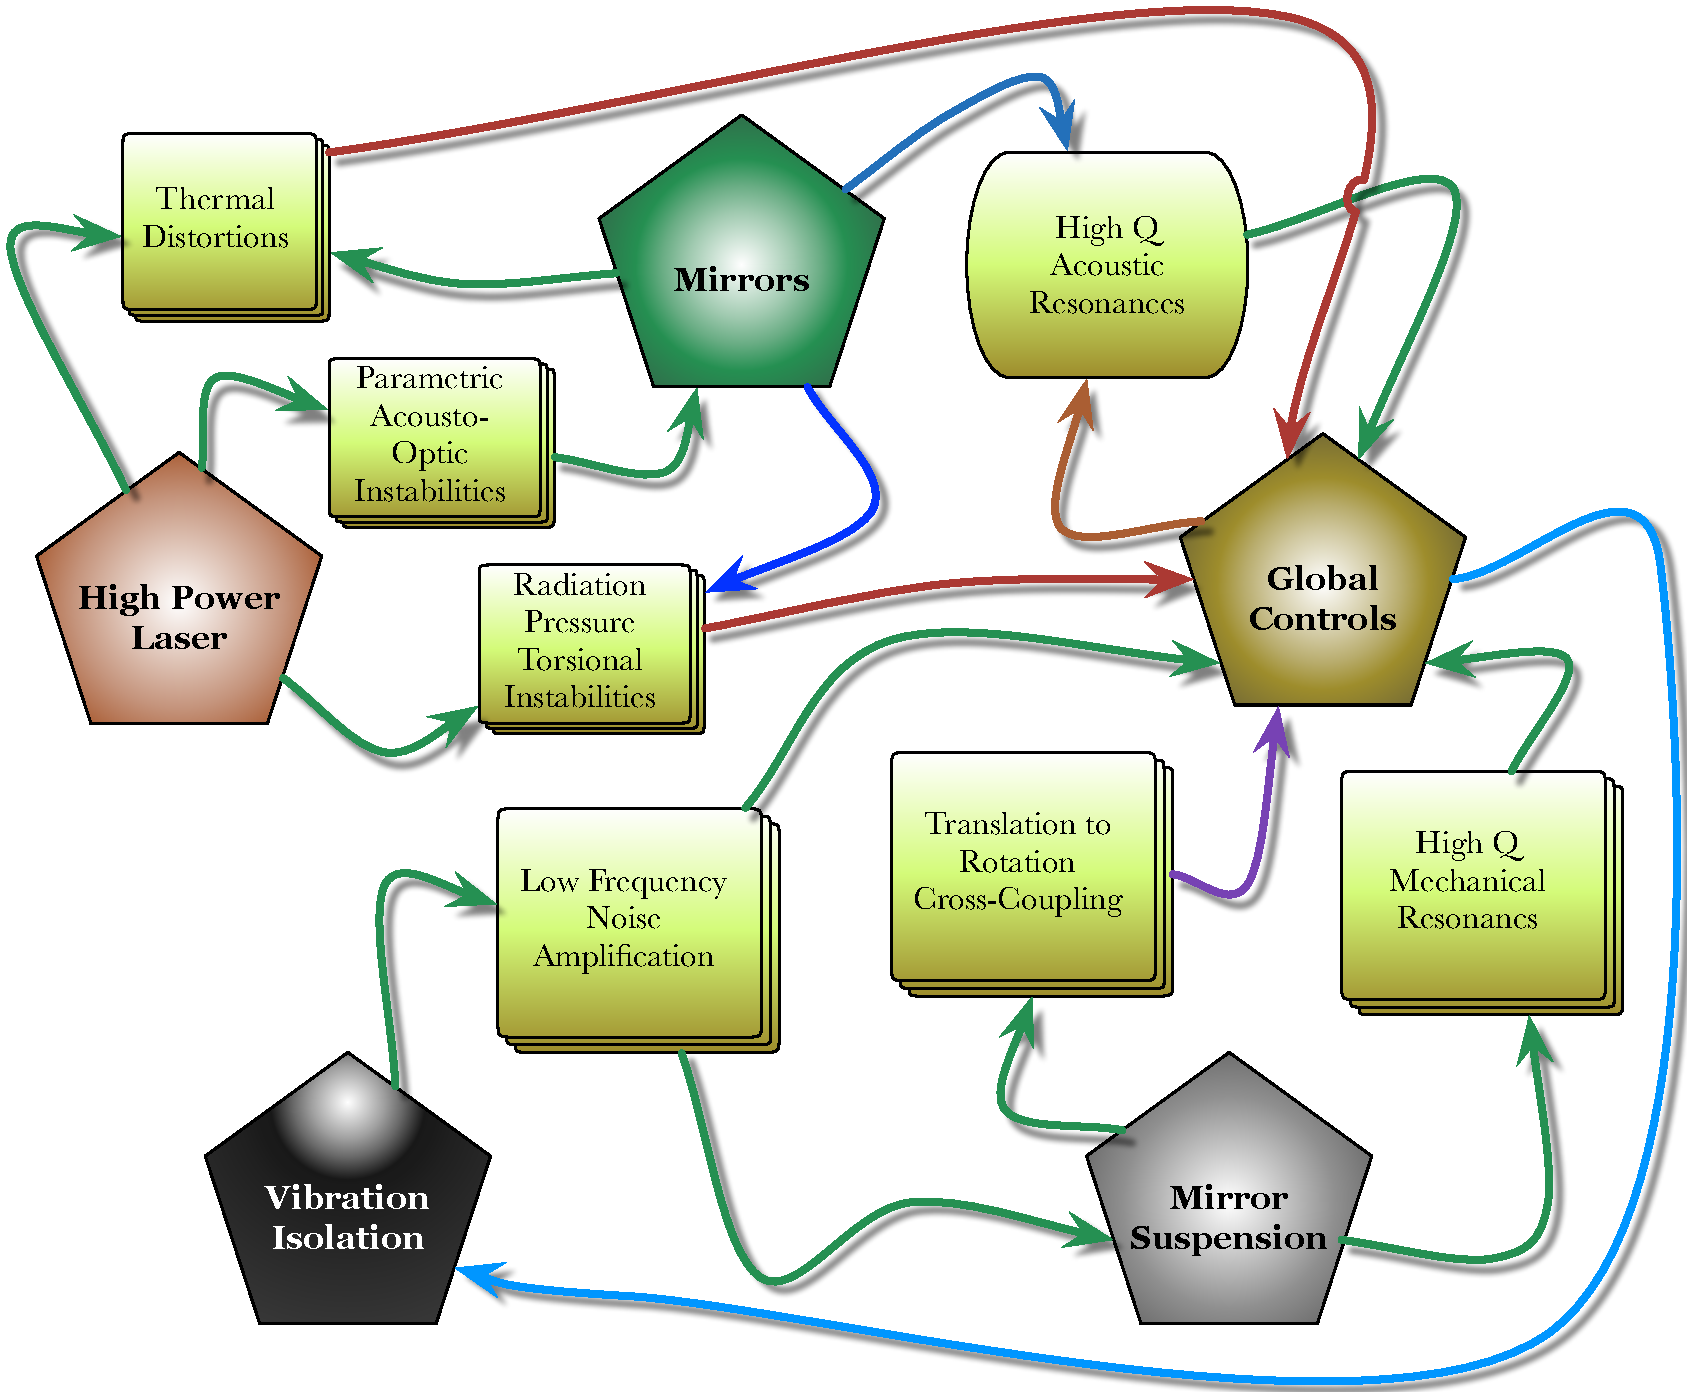
\includegraphics[width=\columnwidth]{Figures/SystemConflicts.pdf}
\caption{Examples of interactions between subsytems}
\label{fig:SystemConflicts}
\end{figure}

Figure~\ref{fig:SystemConflicts} shows diagrammatically many of the most
significant subsystem conflicts/intercations.

\subsection{Issues due to High Laser Power}
To increase the phase (and thereby strain) sensitivity of the interferometer
the circulating laser power in the interferometer is increased (into the MW
regime). This has several problematic consequences:
\begin{itemize}
\item Quantum fluctuations of the radiation pressure increase as P$^{1/2}$, increasing the low frequency strain noise.
\item The classical radiation pressure force due to the high cavity power
leads to static and dynamic instabilities in mirror
orientations~\cite{Sidles:2006un, Dooley:13, aLIGO:ASC}. In addition to producing
more mirror motion, the concomitant increase in the angular feedback
control bandwidth (cf.~Chapter~\ref{ASC}) injects noise into the GW strain
channel at low frequencies (cf.~Fig.~\ref{}), masking the presence of intermediate mass black holes.
\item In addition to angular instabilites, the system of compound resonant cavities can exhibit instabilities along the optical cavity axis~\cite{SGLMW2004, BuCh2002, Osamu:spring}. This
unstable opto-mechanical eigenfrequency can show up in the GW detection band,
making the control system challenging to design (cf.~Chapter~\ref{LSC}).
\item Through the finite optical absorption in the mirror substrates and the
high reflectivity mirror coatings, heat is deposited in the mirrors and thermal
gradients are formed. These lead to thermal lensing and thermal deformations
(cf.~Chapter~\ref{TCS}) which can reduce the stored power in the system, destabilize
the MIMO angular control system, increase the coupling of laser ampltidue and
frequency noise to the strain channel, spoil the dark fringe contrast, and
aggravate opto-acoustic parametric instabilities (cf.~Chapter~\ref{SYS}).
\item Light which scatters out of the main interferometer and then returns after interacting with a vibrating piece of the environment, will be phase modulated by the vibration. In a low power interferometer, this will just produce phase noise, but depending upon the relative phase of the interferometer field and the backscattered light, this can also produce amplitude noise. These amplitude fluctuations (via radiation pressure) can produce as much as an order of magnitude more strain noise than mere phase fluctuations.

\end{itemize}

\begin{figure}[h]
  \centering
    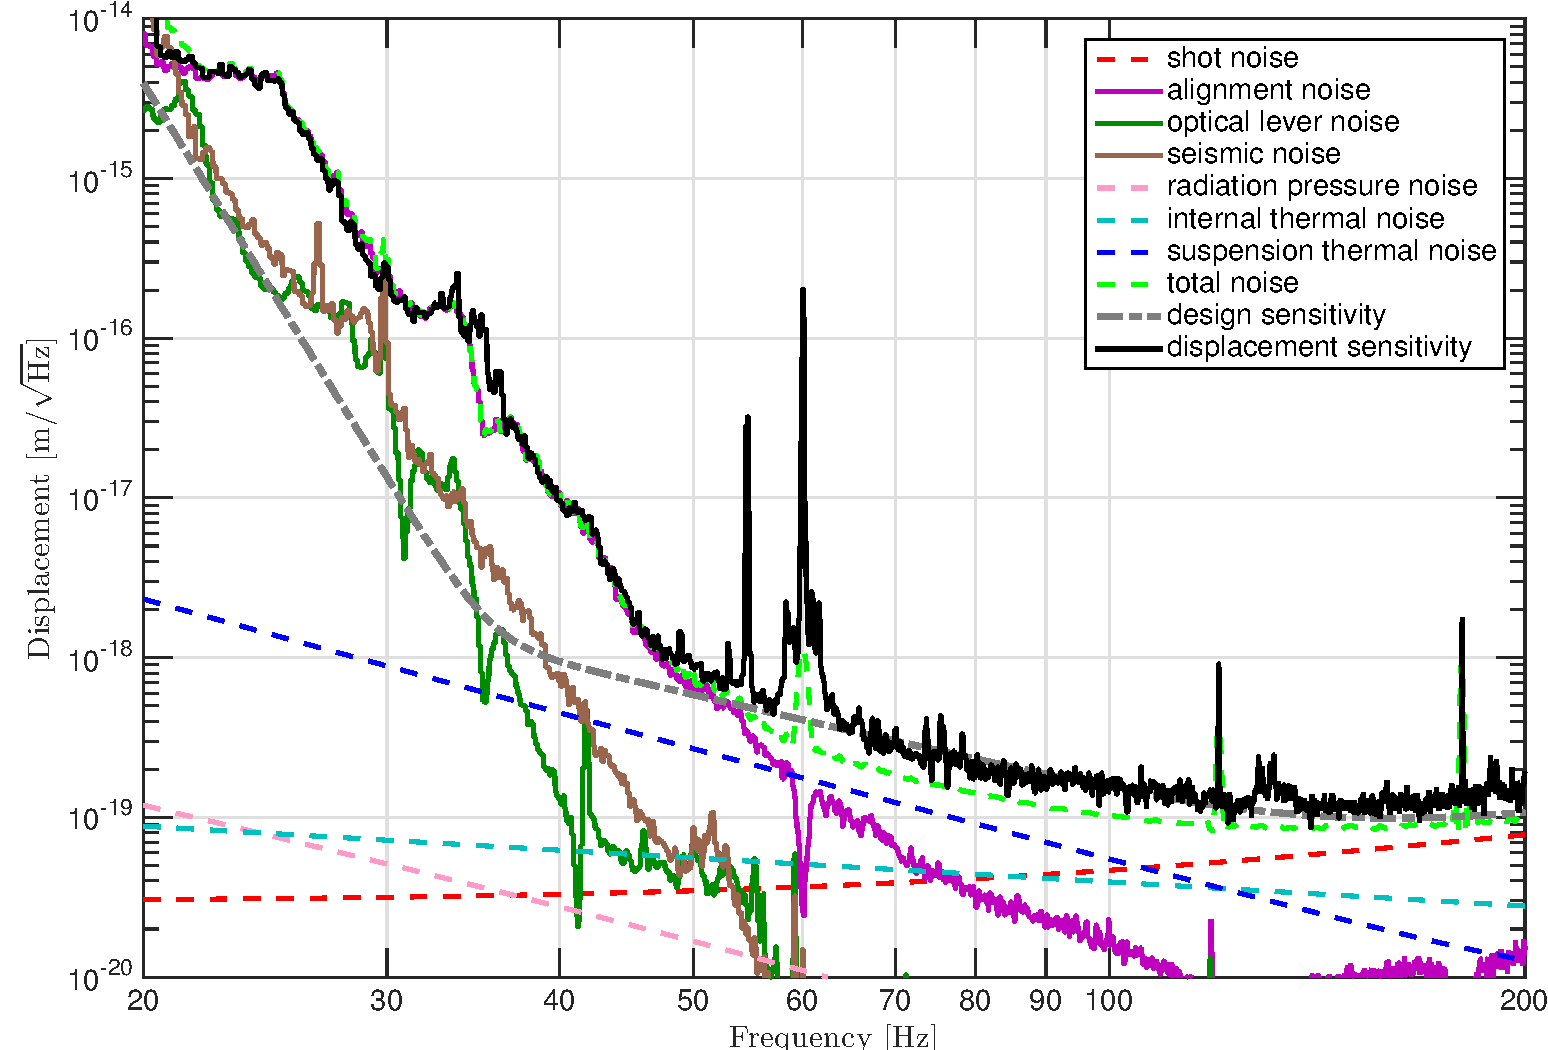
\includegraphics[width=\columnwidth]{Figures/S6_NB.pdf}
    \caption{Contribution of Alignment noise to the noise budget of the
    Enhanced LIGO interferometer in Louisiana (2010)}
    \label{fig:eLIGO}
\end{figure}

\begin{figure}[h]
    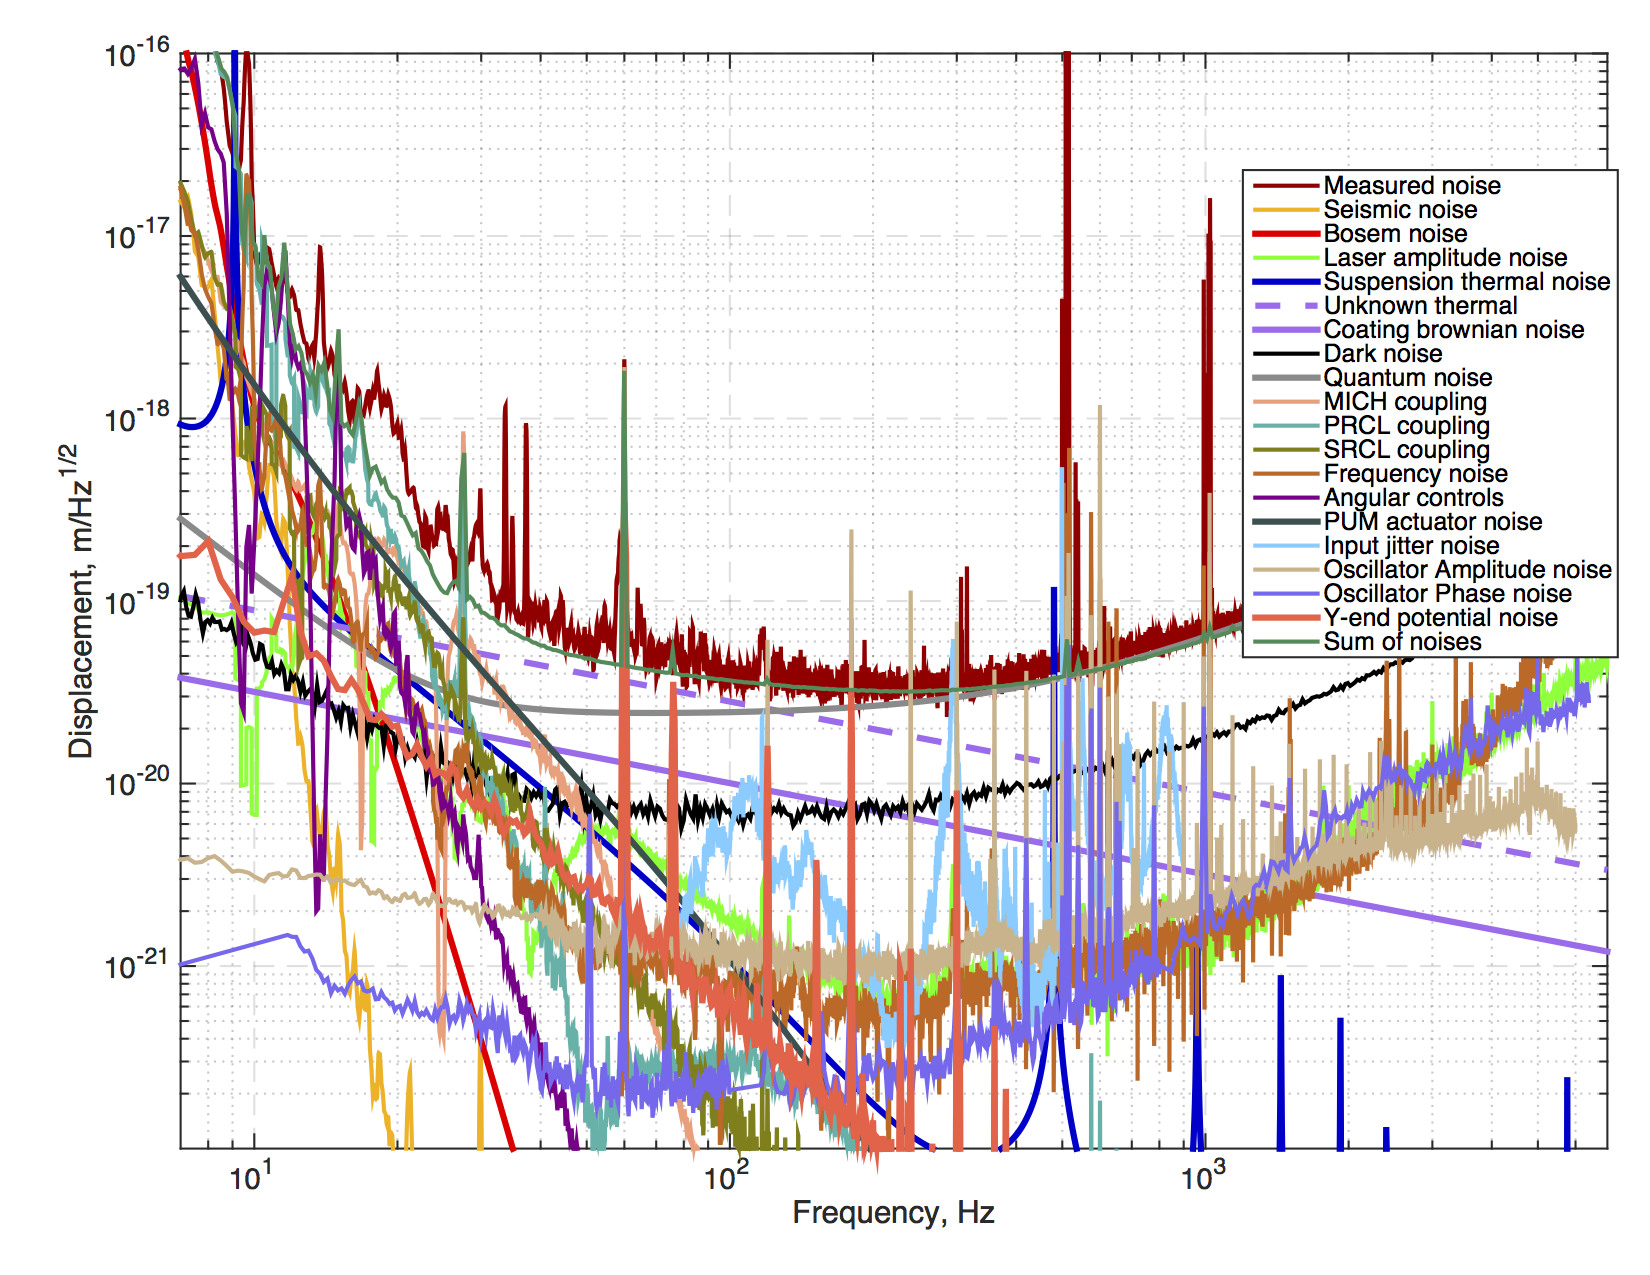
\includegraphics[width=\columnwidth]{Figures/darm_nb.png}
    \caption{Contribution of Alignment noise to the noise budget of the
    Advanced LIGO interferometer in Louisiana (2015): replace with simple plot}
    \label{fig:aLIGO}
\end{figure}


\subsection{Interaction of Mirror Suspension with Global Controls}
The vibration isolation and mirror suspension systems are designed so as to
provide much attenuation of noise at higher frequencies and some (unwanted) amplification
at lower frequencies (cf.~Figure\,\ref{fig:SeismicTFs}). This condition is analogous to the
one encountered in analog electronic filter design:  a sharp transition from
the passband to the stopband requires complex poles in the passband (e.g.
in Chebyshev filters) which amplify the signals at those frequencies. This
is ameiliorated somewhat through the use of 'cold damping'
techniques~\cite{Kuroda:1982vf, Forward:1979ks, Shapiro:2015di}.


\begin{figure}[h]
\centering
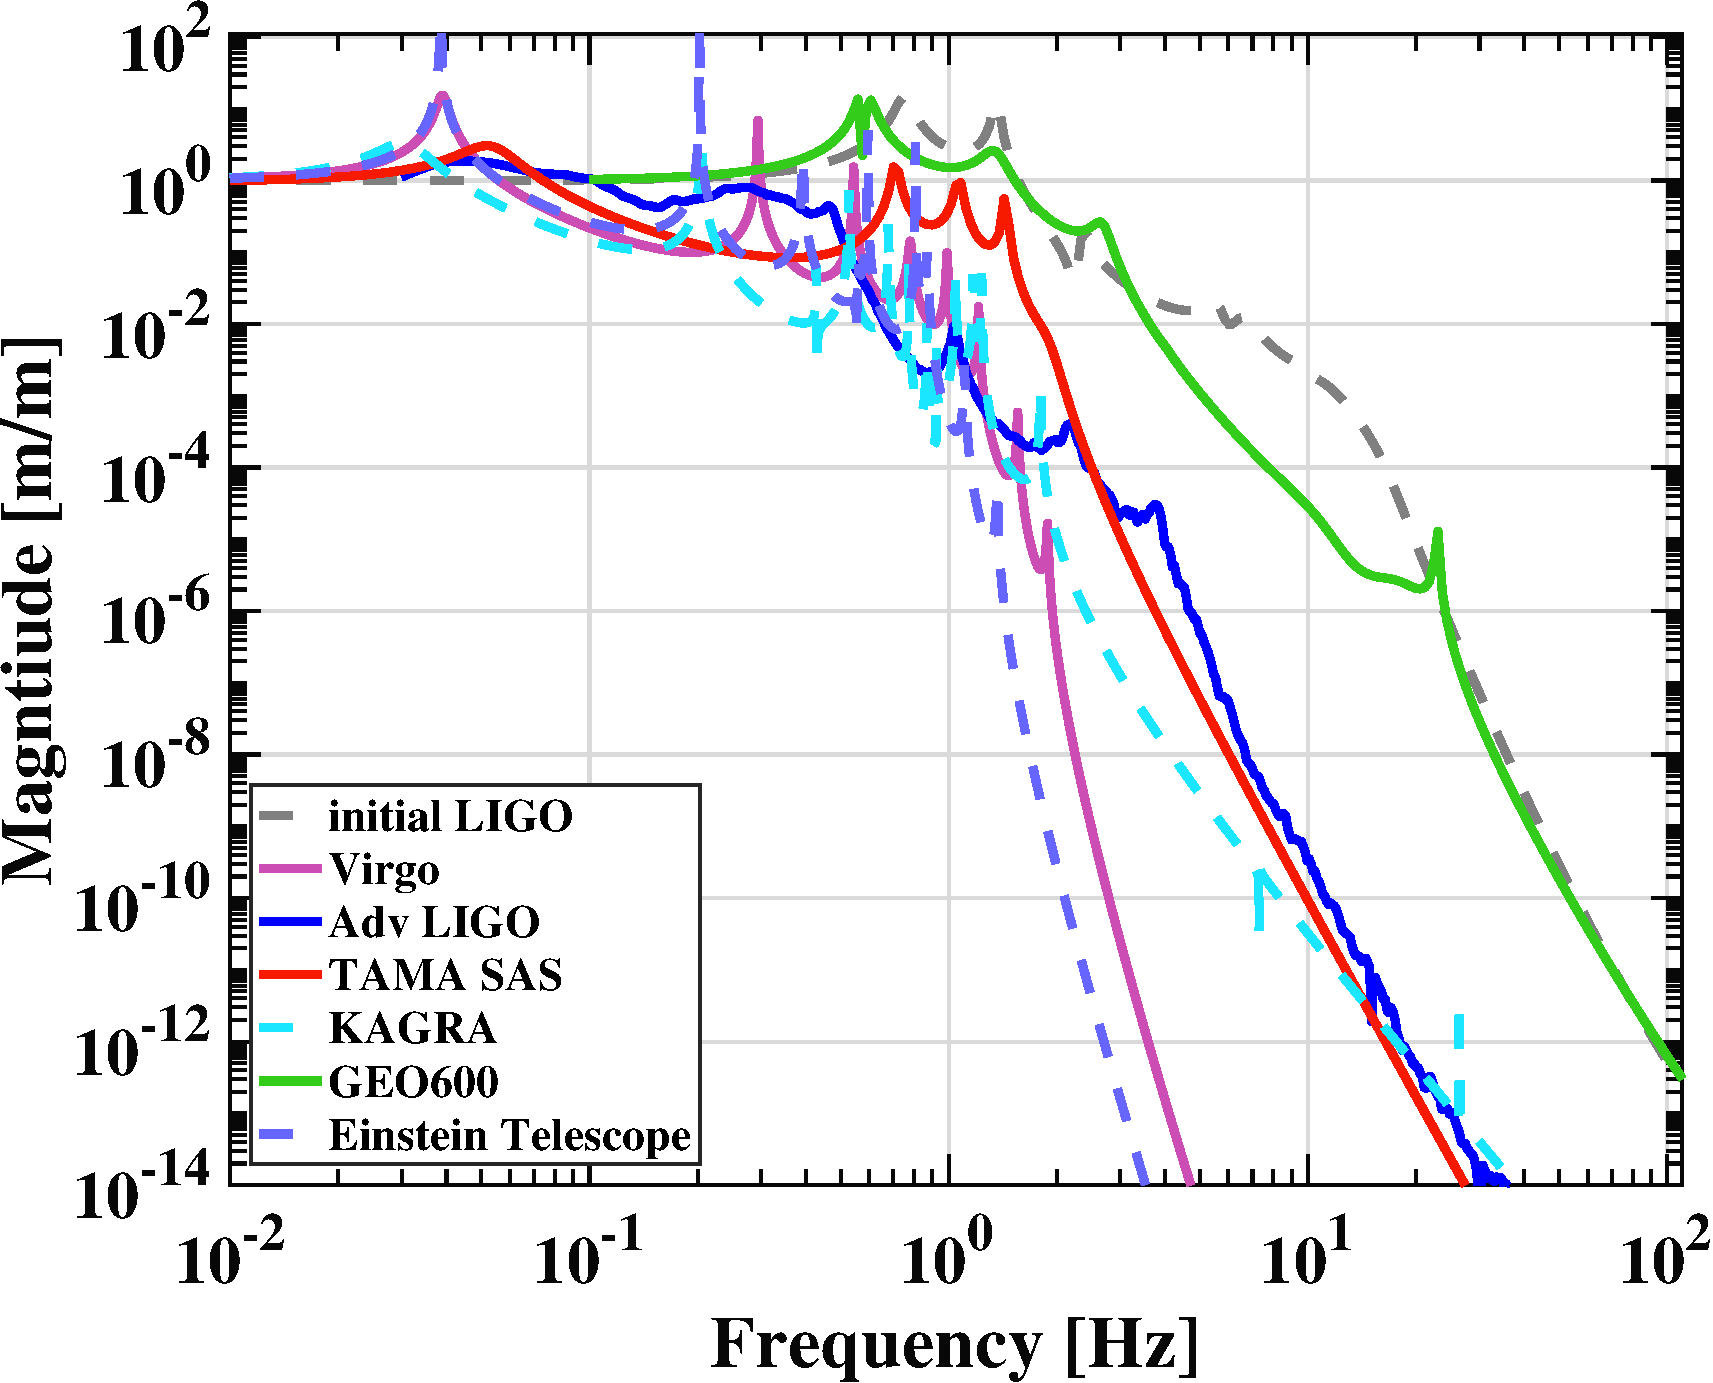
\includegraphics[width=\columnwidth]{Figures/SeismicIsolations.pdf}
\caption{Vibration isolation for the initial LIGO~\cite{ponslet:432, Giaime:1996},
        Virgo~\cite{Stefano:2001, Virgo:SA2010, Accadia:2011jh},
        TAMA (with SAS)~\cite{Szabi:TAMASAS},
        GEO600~\cite{Hartmut:PhD, Ken:GEOseismic, plissi:3055},
        Adv. LIGO~\cite{aLIGO:Seismic2002},
        KAGRA~\cite{Somiya:2011tb}, and the
        Einstein Telescope~\cite{ET2011}. In the KAGRA case,
      the mechanical links for cooling (included) are expected to limit the
      isolation performance above $\sim$\,1\,Hz~\cite{Takahashi:email}}
\label{fig:SeismicTFs}
\end{figure}


Important considerations in test mass suspension design\cite{SUS:2012, Aston:2012}:
\begin{itemize}
   \item Vibration isolation: nearly all of the seismic isolation in the GW detection band ($f > 5\,\rm Hz$)
     comes from the suspension. To fulfill this requirement, the mirror must be isolated by a
     multi-stage pendulum~\cite{Beker:2011}.
    \item low suspension thermal noise and minimization of creep noise~\cite{Levin:2012ek, Gretarsson:2005gs}
    \item third priority is some thoughts on damping
    \item 4th priority is minimize damping noise
    \item should instead consider upconversion, control forces, gradual noise reduction, minimization of angular noise generation, etc. all together in holistic metric v. sensitivity and uptime.
    \item Future suspension will look different than the LIGO/Virgo style
\end{itemize}

\subsubsection{Cross-Coupling of Translation to Rotation}
During the commissioning of the first generation of kilometer scale detectors, it became clear that the angular motion of the suspended optics was too large and a significant challenge for the angular control systems~\ref{ASC}. The most obvious mechanism to produce rotations of the optics is, perhaps, direct coupling of the ground motion through the suspension system and into mechanical torque. However, the rotations of the ground are much too small, when propagated through the pertinent mechanical transfer functions, to explain the observed angular motion.

In fact, the dominant coupling mechanism is due to an interaction between the control system and the off-diagonal elements of the suspension: rotations and translations of the ground produce relative motions of the mirrors along the direction of the laser beam propagation. The Length Sensing and Control (cf.~Chapter~\ref{LSC}) system then corrects for this by applying forces to the mirror suspension system.

The mechanical cross-coupling in the suspension system is so large that this force to angle term dominates over all others. This length to angle coupling has a complicated transfer function from each length actuator to the mirror angle due to the many resonances in the suspension, the presence of the local damping loops, and the Sidles-Sigg effect~\cite{Sidles:2006un, Hirose:10, Dooley:13}. For years, attempts have been made to mitigate this effect by taking the applying a filtered version of the length control force as a torque to the suspension actuators. In the asymptotic low and high frequency regimes, the cancellation achieved by this technique can be as good as 99.9\% or more,
but in the 0.3\,--\,3\,Hz band, where most of the mechanical resonances are,
this drops to only 80\,--\,90\%. The fidelity of this cancellation technique is limited by the required accuracy of the measurements, the slow time variation in the opto-mechanical plant, and limitations in inverting high Q zeros of the mechanical transfer function.


\subsubsection{High Q Eigenmodes}
In the effort to make a mirror suspension with very low thermal noise, the mechanical
elements nearest the mirror must have a very high mechanical Q
(cf.~Chapters~\ref{THN} and \ref{SUS}).
In the ideal steady-state, these modes are driven only by the thermal energy
dictated by the Equipartition theorem and their presence in the data can be simply
removed through standard techniques~\cite{Allen:1999wy, Finn:Violins, Searle:2003ib, Sintes:1998gq}.

Nature, however, is not so kind. Large seismic transients and instabilites in the control systems can lead to large excitations of these modes. The vertical and roll (rotation about the cavity axis)
modes of the mirror suspension fall in the lower end of the observation band
(f $\simeq$ 10-20 Hz) and the higher frequency fiber modes which have nodes at
their endpoints are at multiples of $\sim$\,500\,Hz. The lower frequency modes have
decay time constants of order several hours, whereas the higher frequency ones
have time constants of several days.

Each of the four test masses has a vertical mode, a roll mode, and $2n$ fiber modes
for each of its four fibers. So the total number of high Q suspension modes is:
\begin{equation}
N_{high} = 4 \times (1 + 1 + 4 \times 2n)
\end{equation}
which totals to $104$, if we consider the first few harmonics only.

In order to allow the interferometer to operate, numerous digital feedback
loops have been designed to damp these modes~\cite{martynov2015lock, Miller:ESD}. In the
installed systems, the only way to damp these modes is to sense their perturbation
of the mirror motion and apply feedback forces to the suspension chain. In the case
that thermall induced drifts cause the mode frequencies to overlap, the problem
becomes intractable results in massive downtime of the detectors. Future designs
may utilize dedicated hardware solutions to apply damping forces without degrading
the thermal noise~\cite{Dmitriev:2010hk, Lockerbie:2011zma}.

Ultimately, we have seen that it is not wise to have high Q mechanical modes which are nearly invisible to the control systems. The cost, in terms of time spent developing an ad-hoc solution, is quite high.

%\subsection{Digital Control Systems: A second example}

% ​\section{Control System Synthesis}
%   1) LIGO/Virgo/GEO done by pre-1980 controls technology: pole/zero placement, SISO error signal minimization, by-eye estimates of loop stability
%   2) Techniques for process and aircraft control use more global and MIMO synthesis techniques with general cost function minimization.
%   3) Machine learning techniques can use nonlinear cost functions and account for rare, large excursions -> maximize uptime

% In recent years, more sophisticated algorithms have been introduced to
% better control the vibration isolation
% systems supporting the mirrors in the
% interferometer~\cite{Beker:2014, Driggers:2012fl, Ryan:FFW2012}

%   4) Adaptive machines can explore non-intuitive noise cancelation techniques​
%   5) The dynamical response of the interferometer is a combination of mechanical, opto-mechanical, and electronic feedback. Its a mistake to treat these on such unequal footings - the interferometer design ought to be done using global search methods (such as MCMC) in the same way that we do for BHBH parameter estimation.






% \section{Most Surprising Noise Sources}
%
% \begin{itemize}
%   \item Classic bilinear: beam spot motion makes upconversion. Well understood in the 90's.
%   \item Limiting noise in S1: seen, but not understood until S2.
%   \item Weak LO: limit in S3. Found by noticing harmonics in spectra. Same structure as S1 OL noise.
%   \item Multiple PDs: the signal is not the same.
%   \item RF AS PD: What's in the I-phase?
% \end{itemize}


\subsection{Scattered Light}
\label{s:IDC:scatter}
The sensitivity required to make gravitational wave measurements can be expressed also
as a sensitivity to \textit{optical phase} fluctuations. The current state of the art
is approximately $10^{-11}$ radians/$\sqrt{\rm Hz}$ and is nominally considered to be limited
by quantum mechanics and the available laser power~\ref{SQN}. Practically, however,
all of the high sensitivity interferometers in the past 30 years have been limited
at some frequencies by the non-fundamental phase fluctuations due to scattered light.
This phenomenon of excess phase
noise due to scattered light has been known about for decades~\cite{Schilling:1981}
but the methods by which to combat it have been developing steadily since then and
involve the highest levels of experimental artistry in the field of laser interferometry.

Due to imperfections in the optics, for example, a small fraction of the laser light escapes from
the main interferometer beam path. This light then interacts with something (e.g. a piece of the
vacuum system or some other suspended optic or beam dump) and then recombines with the
circulating laser field within the
interferometer~\cite{Kip:Scatter95, Kip:scatter1989, Sam:Scatter2012,
Stefano:Scatter, vinet1997scattered, fritschel1998high}.
The recombination may occur at virtually any point within the system: inside of the
Fabry-Perot arm cavities, at the beamsplitter, or even at the final photodetector which
records the GW strain signal. Scattered light induced phase noise in the sensing
of auxilliary degrees of freedom can couple into the strain channel through the
relevant feedback control systems~\ref{LSC, NFN}.

It is instructive to consider quantitatively the ampltidue of the noise for a few of
these cases.
\subsubsection{Case I: The Beam Tube Baffles}
Let us assume in this case that the field scatters from the test mass surface,
reflects from a piece of multi-km long beamtube, returns to the same test mass
mirror, and then recombines into the circulating cavity mode. The resulting electric
field fluctuation will be
\begin{equation}
\delta u_{s} = \frac{4 \pi}{\lambda} x_{s}(f) P_s^{1/2}
\end{equation}
For comparison, the field fluctuation due to mirror motion will be
\begin{equation}
\delta u_{m} = \frac{4 \pi}{\lambda} x_{m}(f) P_0^{1/2}
\end{equation}
where $x_s$ is the motion of the beamtube in the direction of the mirror, $x_m$
is the motion of the interferometer mirror, $\lambda$ is the laser wavelength,
$P_0$ is the power stored in the arm cavity, and $P_s$ is the power which
recombines into the circulating cavity mode. Ignoring for a moment the radiation
pressure effects, we can see that the phase noise due to this type of backscatter
can be simply expressed (in units of mirror displacement) using the ratios of
the stored power and the backscattered power. The recombined power is
\begin{equation}
\frac{\delta P_s}{P_0} = \frac{\lambda^2}{r^2} \left( \frac{dP}{d\Omega_{mb}}\right)^2 \frac{dP}{d\Omega_{bm}} \delta \Omega_{mb}
\end{equation}


\subsubsection{Case II: The Test Mass Chambers}


\subsubsection{Case III: Backscatter from the Dark Port}


\subsubsection{Case IV: Backscatter from the Bright Port}
A significant source of scatter for all of the long interferometers
\begin{align}
S_x = some scattering stuff
\end{align}

\subsection{Environmental Noise Sources}
We would like to imagine that since the interferometers are in a vacuum system and
protected from the ground by very sophisticated vibrations isolation equipment,
the coupling of environmental acoustics would be zero. In fact, a host of environmental
disturbances~\cite{Effler:2015hw, Acernese:2006dq} (cf.~Figure~\ref{fig:EnvironmentalNoise}) show up in the interferometer
output (or are expected to in future detectors) at a level much higher than
expected by the Navier-Stokes equations~\cite{Greenspan:sound} for low frequency
acoustics at the $\sim10^{-6}~Pa$ pressures of high vacuum experiments. The reason
for this is that the coupling paths are not through vibration of the air molecules
in the high vacuum system, but through the motion of the vacuum chambers and tubes.




\begin{figure}[t]
\centering
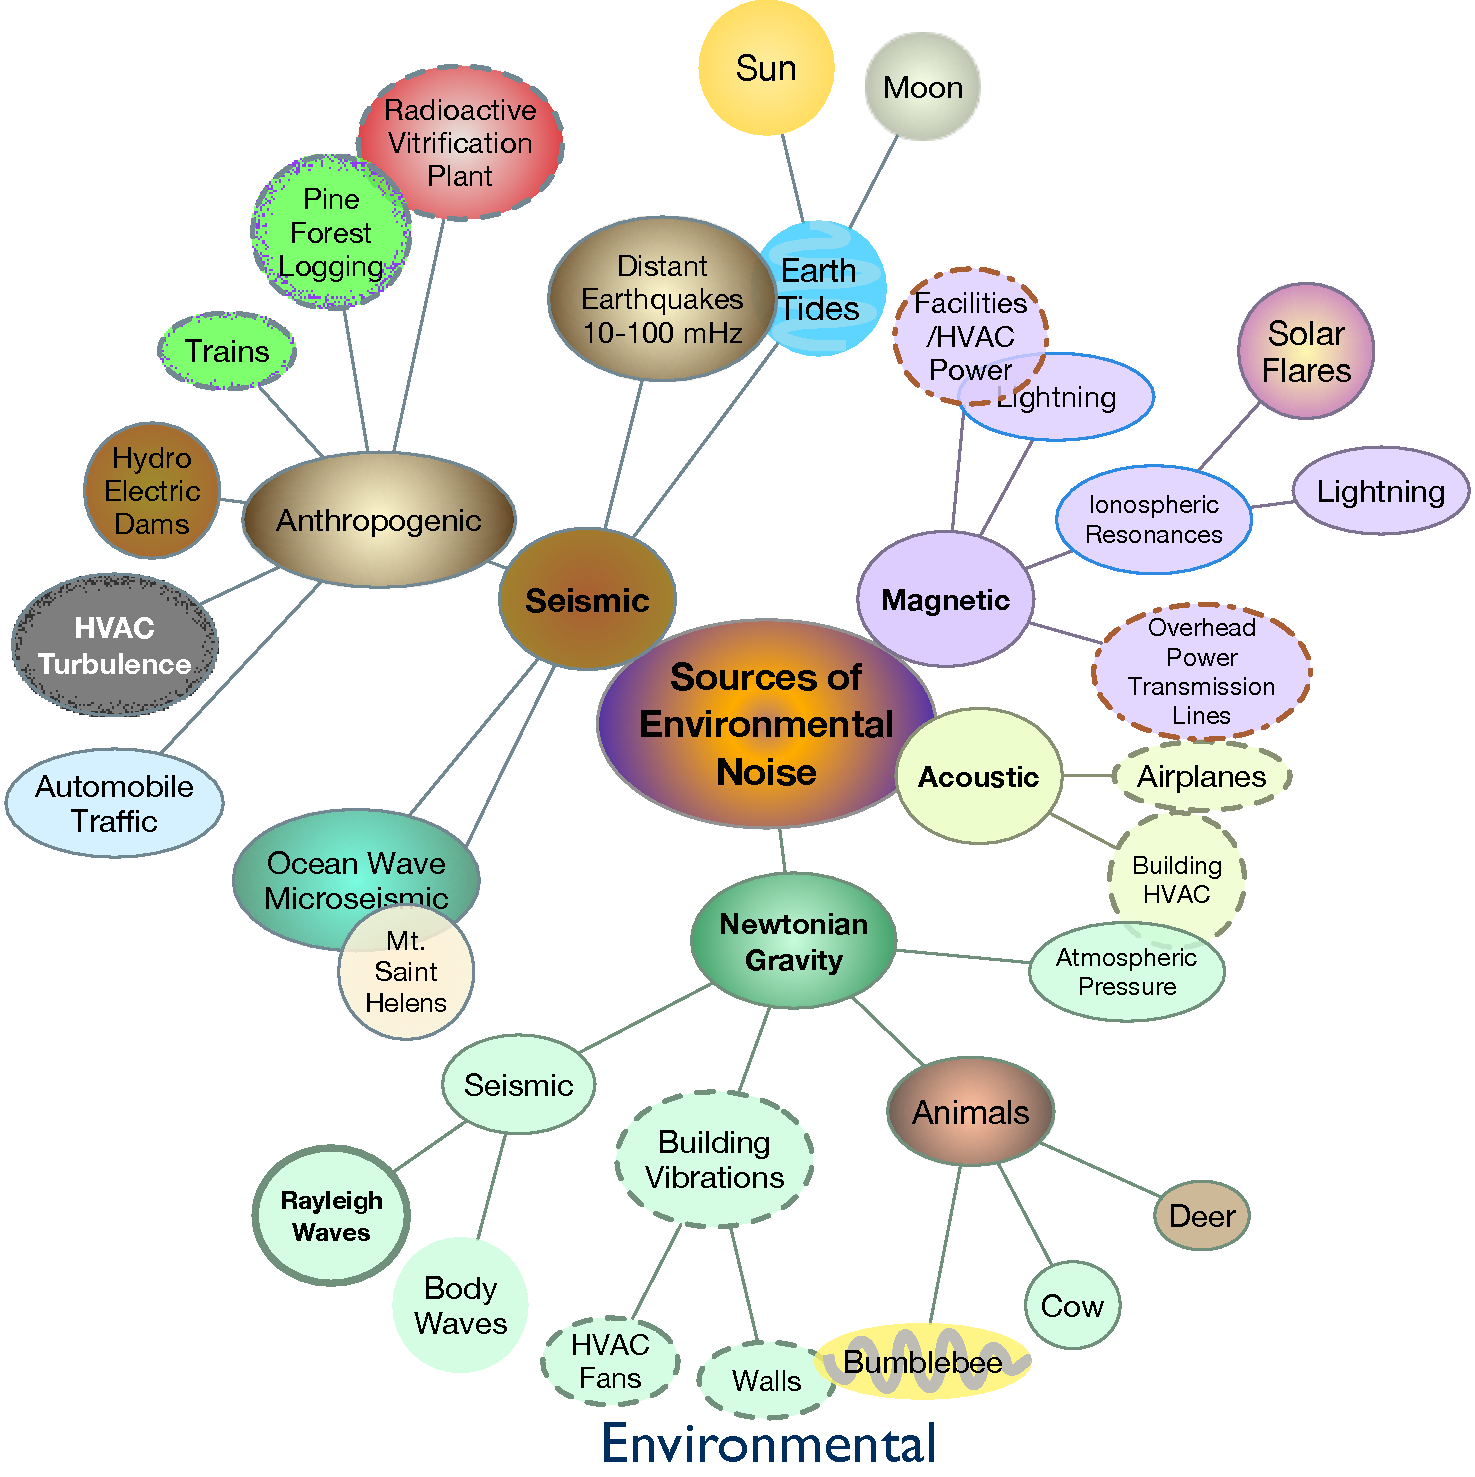
\includegraphics[width=\columnwidth]{Figures/Environmental.pdf}
\caption{Graphical representation of environmental sources of noise. The detector
design nominally isolates against many of these, but some of the sensitivity to,
e.g. acoustics or magnetics, comes in mainly as a consequence of the vacuum
or control system design.}
\label{fig:EnvironmentalNoise}
\end{figure}


\section{Risk Register and Risk Reduction Research}
\label{s:IDC:Risk}
The concept of a Risk Register is common in project management circles and refers
to a log of all the risks know to the project and their associated details. In
the context of the interferometer commissioning and noise hunting, it is a log of
the suspected noise sources, events which might damage some parts of the detector,
and other phenomena that may negatively impact the sensitivity or uptime for
astrophysical searches (such as hurricanes, earthquakes, students leaving, etc.).
While it is not unheard of for such project management tools to give one the
illusion of concreteness and control, the process of looking into the future
for problems to tackle can be very valuable in the long run.

In Table~\ref{t:IDC:Risk} and Figure~\ref{fig:RiskBubbles} an example of such
a register is given for the next several years of Advanced LIGO.

% \begin{table}
% \tiny
% \begin{tabular}{ | l | c | c | c | c | c | c | c | }
% \hline
% 	Risk Description & sub-System & Prob. (\%) & Cost (M\$) & Time (mo) & BNS (\% Range) & BBH (\% Range) & Total Severity \\ \hline
% 	Gravity Gradients & SEI & 75 & 0.3 & 5 & 10 & 90 & 41.6 \\ \hline
% 	Thermal Distortion destabilizes ASC & AOS & 60 & 0.5 & 18 & 30 & 50 & 145.8 \\ \hline
% 	OMC PZT noise & LSC & 15 & 0.1 & 2 & 5 & 5 & 0.58 \\ \hline
% 	LSC Aux noise & LSC & 25 & 0.03 & 3 & 15 & 15 & 4.387 \\ \hline
% 	ASC feedback noise & ASC & 65 & 0.03 & 6 & 5 & 90 & 37.4 \\ \hline
% 	Beamtube Backscatter & SYS & 33 & 0.15 & 5 & 3 & 65 & 11.1 \\ \hline
% 	SRC Mode Healing - Harming & SYS & 50 & 0.5 & 6 & 40 & 5 & 37.3 \\ \hline
% 	BS clipping - contrast defect & COC & 90 & 0.35 & 6 & 33 & 3 & 54.9 \\ \hline
% 	ETM Charge fluctuations & SUS & 50 & 0.2 & 4 & 15 & 40 & 16.2 \\ \hline
% 	Parametric Instabilities & LSC & 70 & 0.2 & 4 & 40 & 5 & 34.8 \\ \hline
% 	Suspension crackle & SUS & 25 & 0.25 & 7 & 5 & 50 & 10.5 \\ \hline
% 	Coating thermal noise anomaly & COC & 20 & 0.75 & 8 & 30 & 3 & 14.8 \\ \hline
% 	OMC backscatter & LSC & 55 & 0.1 & 3 & 10 & 2 & 5.2 \\ \hline
% 	Vac Chamber Acoustics & SYS & 70 & 0.1 & 2 & 10 & 3 & 4.6 \\ \hline
% 	Residual Gas & SYS & 40 & 0.6 & 4 & 30 & 5 & 15.1 \\ \hline
% 	Bounce/Roll modes & SUS & 80 & 0.15 & 3 & 20 & 95 & 34.9 \\ \hline
% 	Violin Modes & SUS & 35 & 0.15 & 3 & 80 & 10 & 26.1 \\ \hline
% 	Control system instability & SEI & 10 & 0.03 & 3 & 100 & 100 & 11.7 \\ \hline
% \end{tabular}
%
% \caption{Example of a Risk Register for the Advanced LIGO detector. This can be used to guide theoretical and experimental risk reduction research. The column headings are
% name of the Risk, sub-system, Probability of occurence within 5 years, hardware
% cost to repair, time to repair (months), \% reduction of binary neutron star range,
% and \% reduction of ($30/30 M_{\odot}$) binary black hole range.}
% \label{t:IDC:Risk}
% \end{table}
\begin{figure}[h]
  \centering
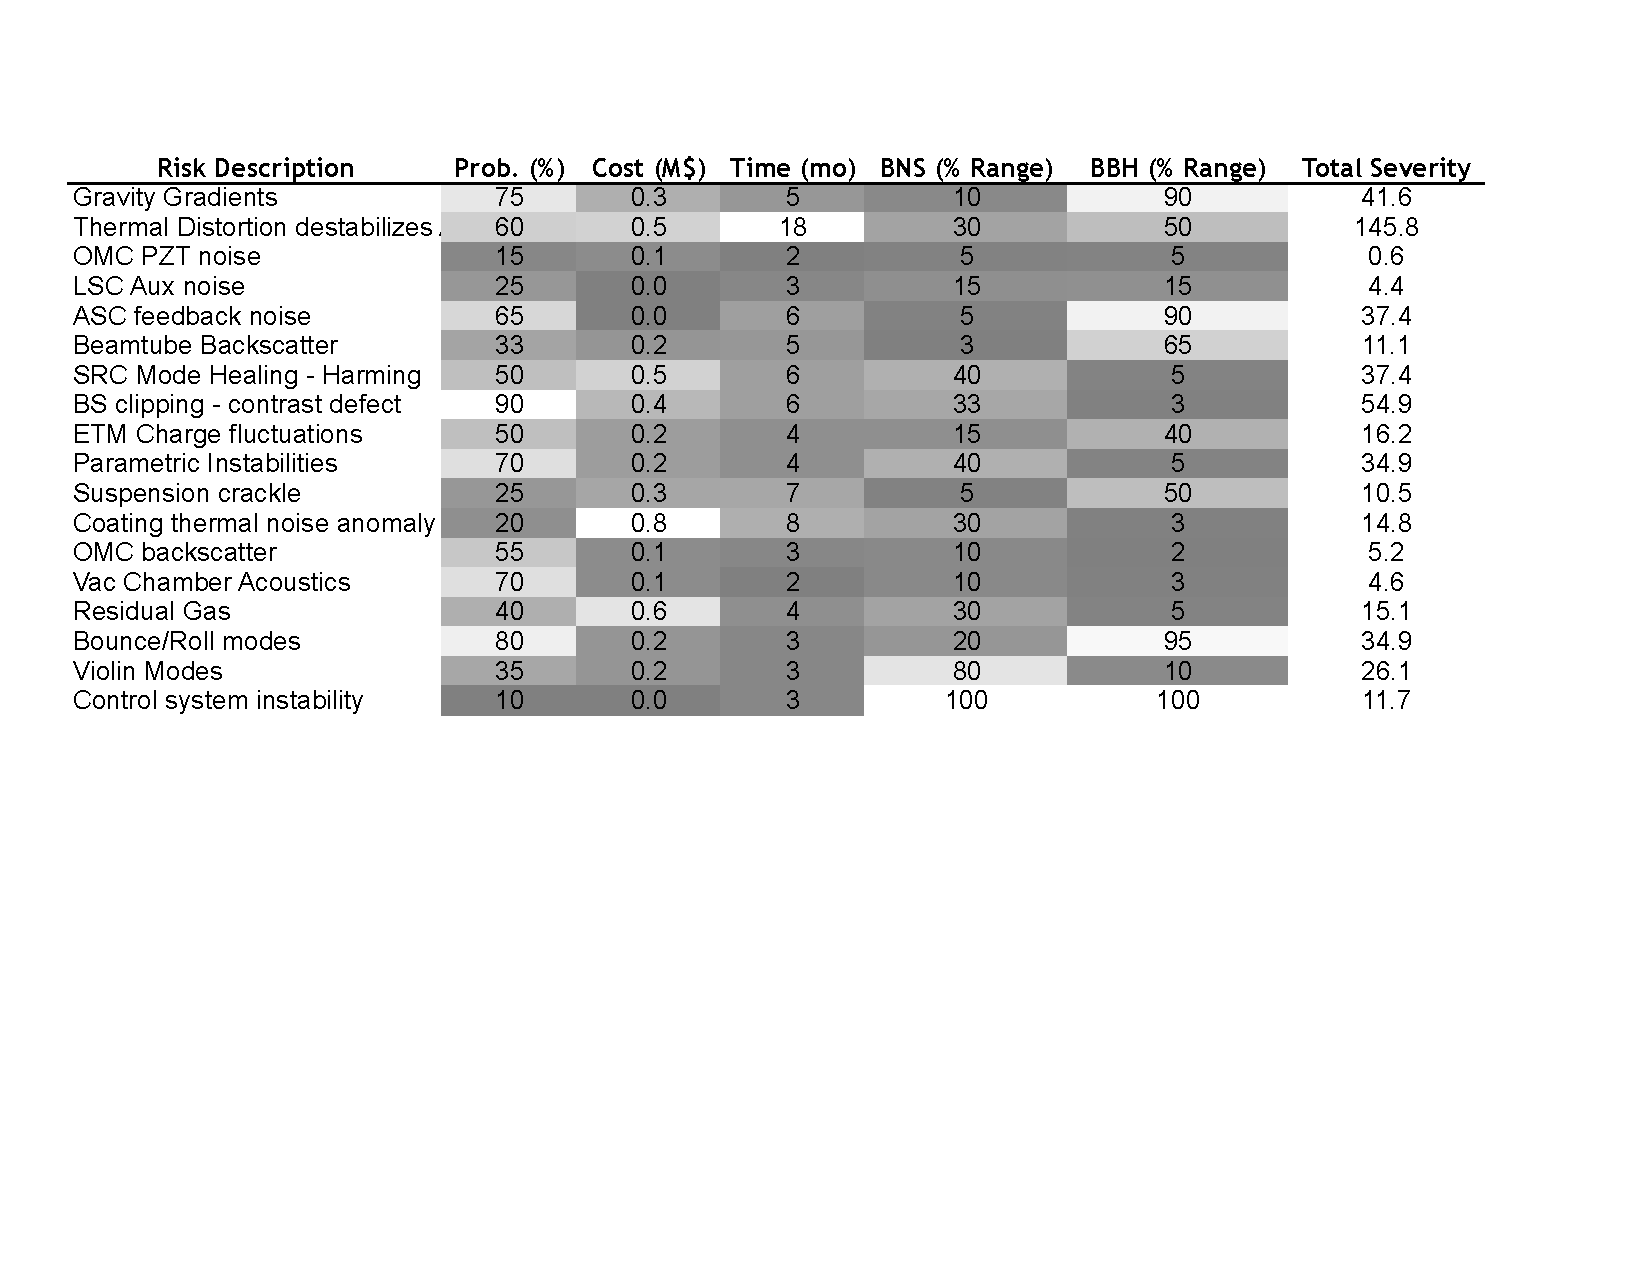
\includegraphics[width=\columnwidth]{Figures/RiskRegister.pdf}
  \caption{Example of a Risk Register for the Advanced LIGO detector. This can be used
  to guide theoretical and experimental risk reduction research. The column headings are
  name of the Risk, sub-system, Probability of occurence within 5 years, hardware
  cost to repair, time to repair (months), \% reduction of binary neutron star range,
  and \% reduction of ($30/30 M_{\odot}$) binary black hole range.}
  \label{t:IDC:Risk}
\end{figure}

\begin{figure}[h]
  \centering
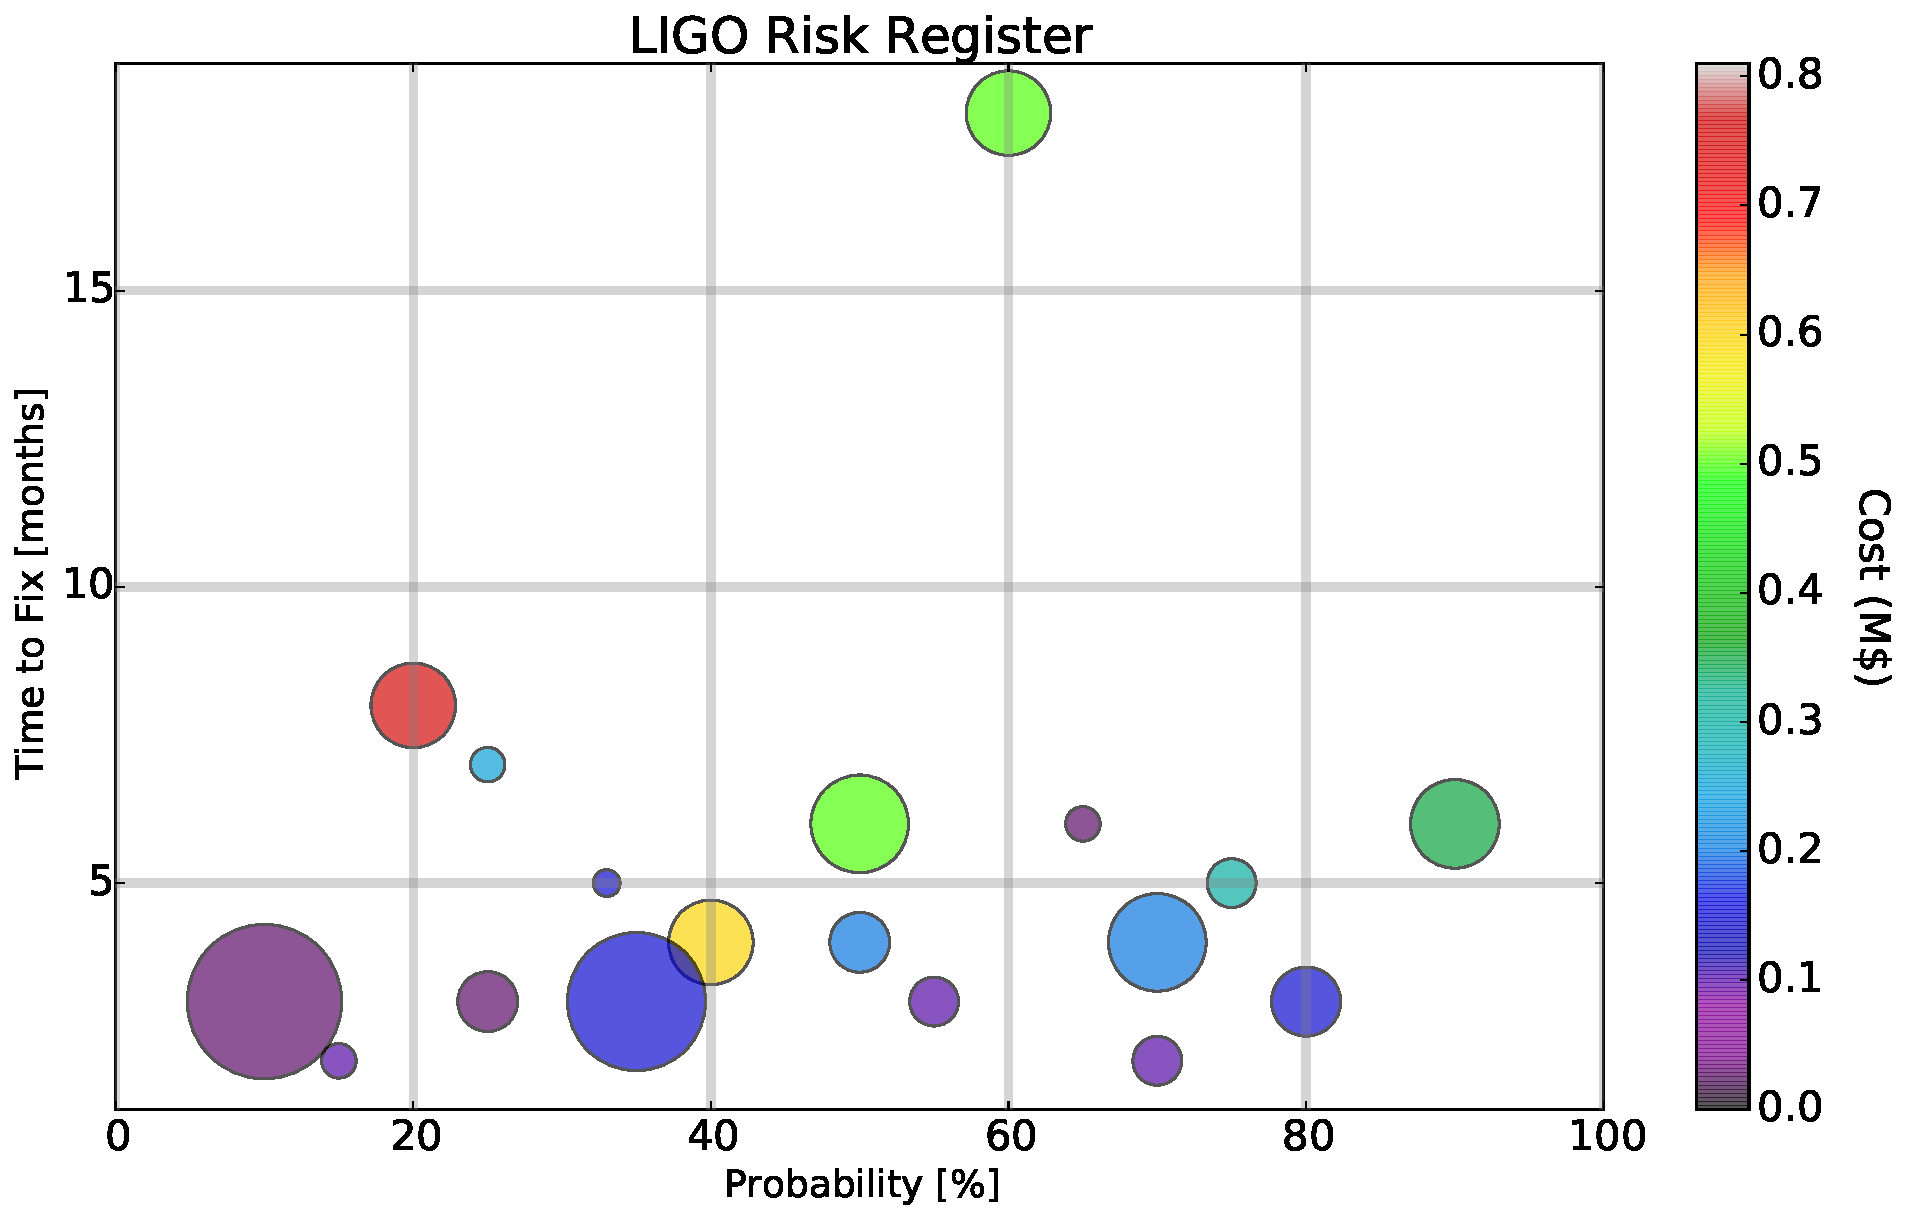
\includegraphics[width=\columnwidth]{Figures/Risk.pdf}
  \caption{Example Risk Register for Advanced LIGO. The area of each circle is
  proportional to the impact on the binary neutron star inspiral rate
  (time $\times$ range$^3$).}
  \label{fig:RiskBubbles}
\end{figure}


\section{Detector Diagnostics}
\label{s:IDC:diagnostics}
During the integration process, it became clear that the addition of numerous
extra diagnostics would make diagnoses of rare problems easier to make. Although
a few of these are in place for some of the detectors (KAGRA, Virgo, LIGO, GEO),
it is fair to say that none of the following have been uniformly implemented and
they are esoteric enough to make this unsurprising.

Since the GW detection band overlaps mainly with the audio band, the
    digital systems which we use to record signals and hunt for noise. The highest
    frequencies that we can monitor are 10\,--\,20\,kHz. In order to diagnose
    excess noise in lasers, electronics, etc. at frequencies of up to several
    MHz we are often forced to move analog equipment around the site and manually
    check for problems. In future detectors, more care should be paid to allowing
    for these diagnostics, either by the use of FPGA based high frequency
    digitizers or by remote access of dedicated analog test instruments.

Chapter\,\ref{COP} describes the higher order spatial modes (HOM) of
    Fabry-Perot optical resonators. Most of the considerations included when
    refining the design of the modern detectors, either consider the frequency
    response of the TEM$_{00}$ mode or the quasi-static behavior of the
    HOMs (cf.~Chapter~\ref{SIM}). During the commissioning
    of the initial LIGO, the unanticipated asymmetries due to the high frequency
    response of the HOMs lead to an unexpected laser noise coupling~\cite{Stefan:Thesis}.
    This situation is complicated by the non-spherical aberrations in the mirrors
    produced by polishing errors, coating non-uniformity, and time dependent
    thermal gradients. These effects all serve to move the HOM resonance frequencies
    slightly from their ideal positions~\cite{Siegman:Lasers}.

In addition to the instabilities caused by the mirror
    suspension (described above), the eigenmodes of the mirrors can be
    excited by the control system, either by the physical mirror actuators
    or through the high bandwidth laser frequency control loops
    (cf.~Chapter~\ref{LSC}) which can apply forces to the mirrors by the
    frequency to ampltiude conversion in detuned optical cavities and the
    resulting radiation pressure force.

The acousto-optic parametric instability~\cite{Matt:PI} control
    systems, by definition, require high frequency monitoring capability
    (cf.~Chapter~\ref{SYS}).

\begin{itemize}
  \item non-uniform optic absorption
  \item time dependence of optical scattering
  \item how close are the optics to the stops
  \item THD of the force actuators
  \item THD of the displacement sensors
  \item strain release in vacuum system couples to IFO by scattered light
  \item bursts of gas lead to transient phase noise in arm cavities
\end{itemize}

\section{People}
\label{s:People}
One of the most important elements in the continuous evolution of gravitational
wave sensitivity is the scientific workforce. These people serve to to do the
hands on work required for the daily progress and later become the leaders
in the field who are responsible for the design and implementation of future
technologies.

This organism needs to be maintained and groomed in an appropriate manner so
as to maximize the long term scientific output of the field. When we use
adaptive filters or machine learning algorithms, we often discuss tuning the
'cost function' in order to guide the algorithm to optimize something. In a
similar manner, there must be a balance in order to make short term progress
as needed while also training the newest students and scientists. To train
a continuous stream of students, suitable PhD projects must be developed
which have sufficient scientific potential. These projects must be
undertaken in a way which allows speedy progress of the interferometers
while simultaneously allowing for the start up training time of students.

\begin{figure}[h]
\centering
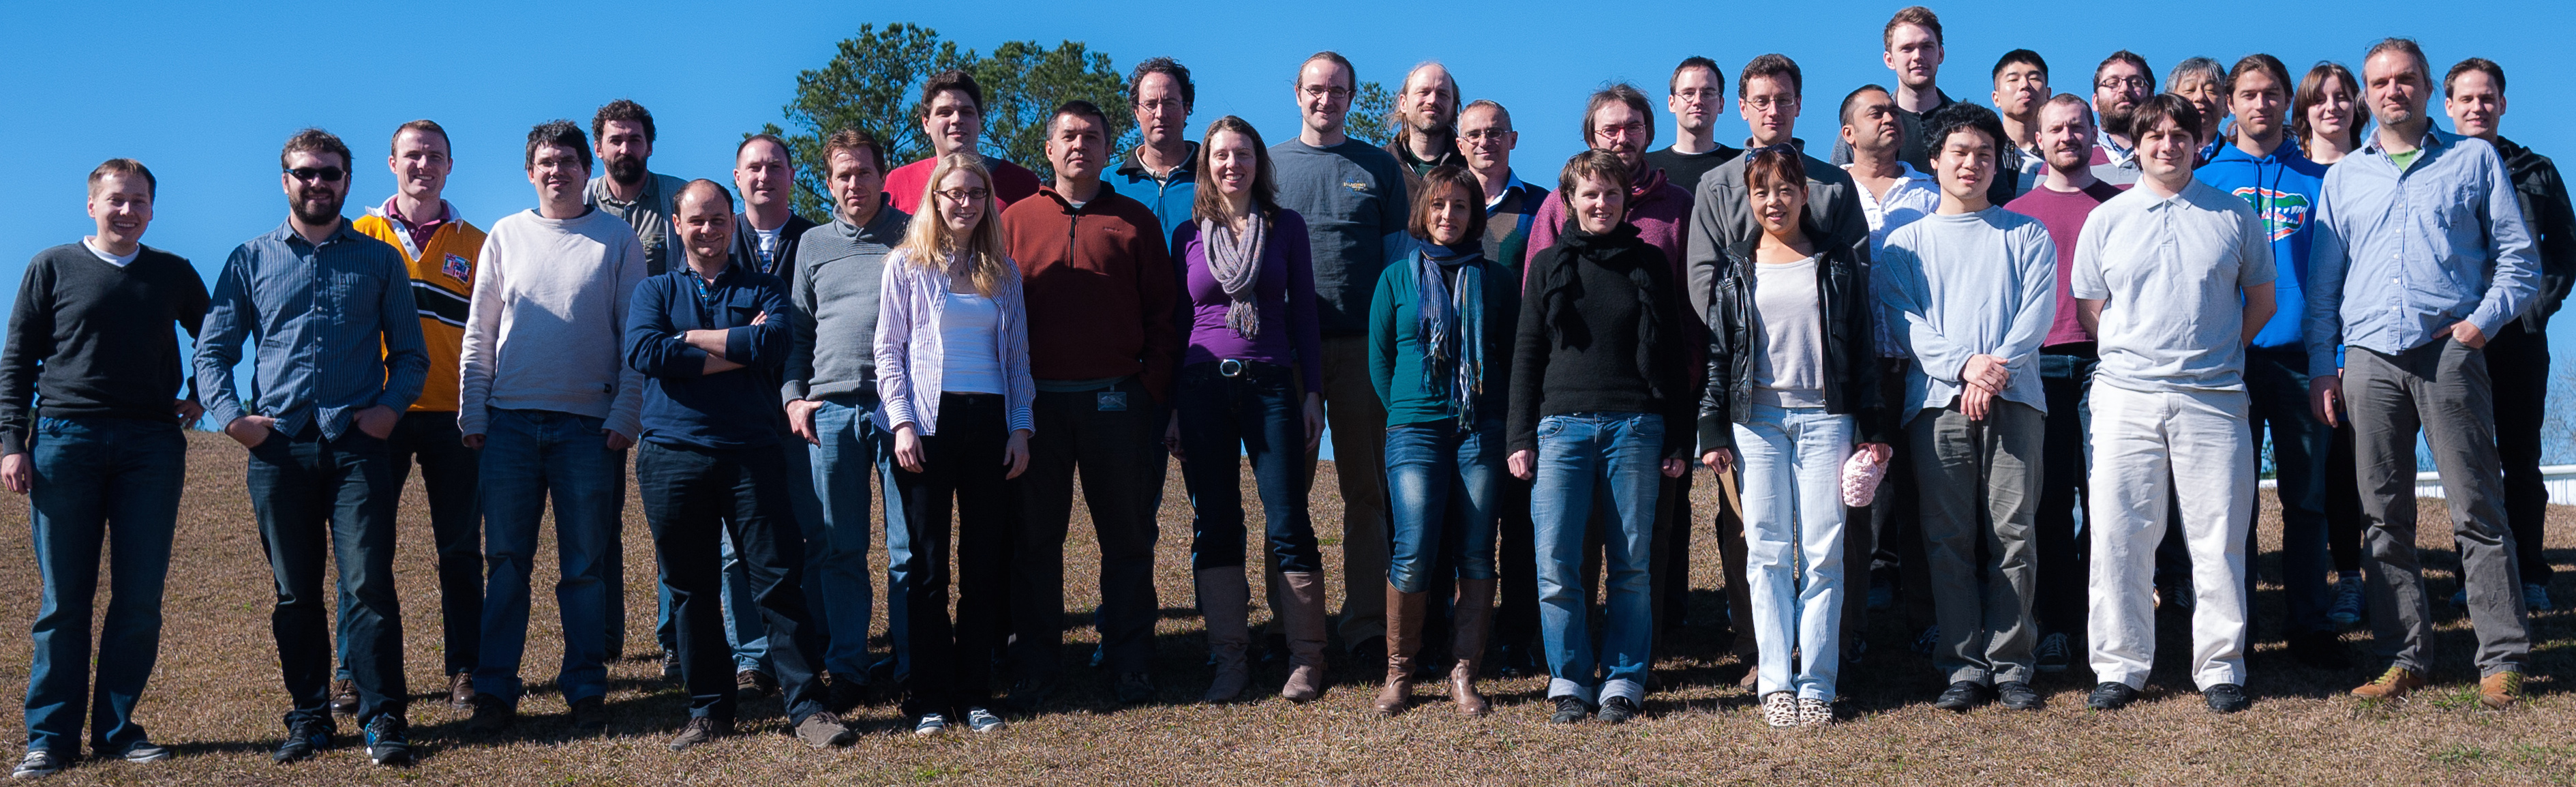
\includegraphics[width=\columnwidth]{Figures/GroupPhoto_LLOworkshop13.jpg}
\caption{International GW Commissioning workshop}
\label{fig:workshopPhotoLLO}
\end{figure}

We don't want students building the detector. Having several inexperienced people
working on the interferometer at the same time can quickly lead to a madhouse
situation.

People need time to fiddle in order to attain deep mastery of the experiment.

Its hard to achieve significant insights without several years of intense
study over all aspects of the experiment.

\subsection{Exchange of Information}
Short term visits not so useful. Long term visits serve to exchange the
technqiues and tricks that we have not thought to publish~\cite{HarryCollins}
and to establish personal relationships which allow the free exchange of
knowledge in the future and make it easy to ask for help.


\section{Conclusion}
These wise things should be kept in mind while doing the detector commissioning.

In addition to the usual thoughts about how to radically improve the detector sensitivity.

Its not possible to think of everything. We need to incorporate the lessons of
the previous generation of detector, while keeping in mind that the design will
be imperfect. How shall we achieve the last order of magnitude in sensitivity
in a rational and deterministic way?

Its important, above all, to stay flexible
and be able to determine when a given system is not functioning adaquetly. At
what point do we decide that the 'hose clamps and duct tape' approach won't
work and we need a professionally engineered replacement for the
malfunctioning component or system or method?
